\documentclass[10pt,a4paper]{article}
\usepackage[utf8]{inputenc}
\usepackage{amsmath}
\usepackage{amsfonts}
\usepackage{amssymb}
\usepackage{graphicx}
\usepackage[left=2cm,right=2cm,top=2cm,bottom=2cm]{geometry}
\usepackage{epigraph}
\usepackage{sfmath}
\usepackage{sansmathaccent}
\usepackage{cmbright}
\usepackage{chemformula,siunitx,chemfig}
\usepackage{color}
\usepackage{tabularx}
\usepackage{hyperref}
\usepackage{cite}


\usepackage[english]{babel}

\DeclareSIUnit\year{yr}

%%%%%%%%%%%%%%%%%%%%%%%%%%%%%%%%%%%%%%%%%
% Formal Text-Rich Title Page 
% LaTeX Template
% Version 1.0 (27/12/12)
%
% This template has been downloaded from:
% http://www.LaTeXTemplates.com
%
% Original author:
% Peter Wilson (herries.press@earthlink.net)
%
% License:
% CC BY-NC-SA 3.0 (http://creativecommons.org/licenses/by-nc-sa/3.0/)
% 
% Instructions for using this template:
% This title page compiles as is. If you wish to include this title page in 
% another document, you will need to copy everything before 
% \begin{document} into the preamble of your document. The title page is
% then included using \titleGP within your document.
%
%%%%%%%%%%%%%%%%%%%%%%%%%%%%%%%%%%%%%%%%%

%----------------------------------------------------------------------------------------
%	PACKAGES AND OTHER DOCUMENT CONFIGURATIONS
%----------------------------------------------------------------------------------------



\newcommand*{\plogo}{\fbox{$\mathcal{PL}$}} % Generic publisher logo

%----------------------------------------------------------------------------------------
%	TITLE PAGE
%----------------------------------------------------------------------------------------

\newcommand*{\titleGP}{\begingroup % Create the command for including the title page in the document
\centering % Center all text
\vspace*{\baselineskip} % White space at the top of the page

\rule{\textwidth}{1.6pt}\vspace*{-\baselineskip}\vspace*{2pt} % Thick horizontal line
\rule{\textwidth}{0.4pt}\\[\baselineskip] % Thin horizontal line

{\LARGE Energy from Biomass : \\ [0.3\baselineskip] Lecture notes \\ [0.3\baselineskip] 22325}\\[0.2\baselineskip] % Title




\rule{\textwidth}{0.4pt}\vspace*{-\baselineskip}\vspace{3.2pt} % Thin horizontal line
\rule{\textwidth}{1.6pt}\\[\baselineskip] % Thick horizontal line

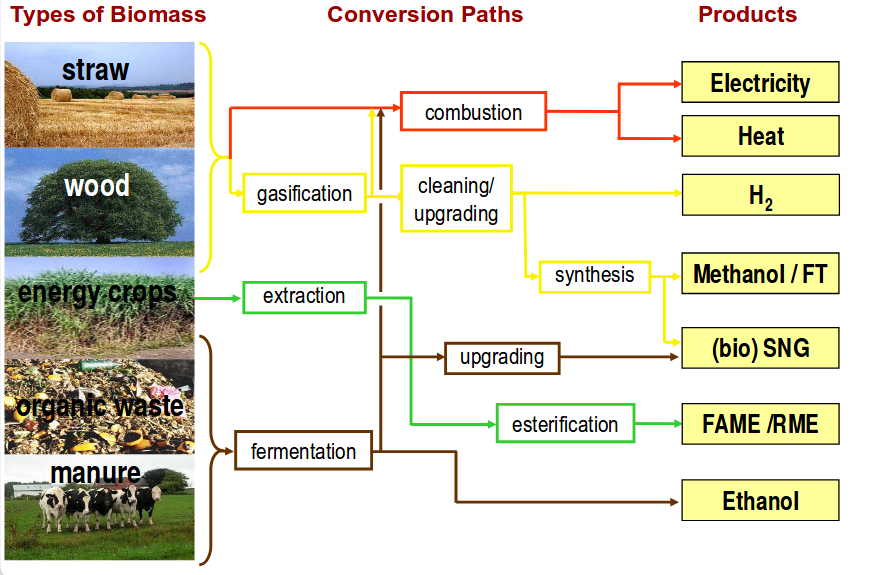
\includegraphics[width=\textwidth]{Image/cover.png} 

\scshape % Small caps
%Travail de réflexion critique sur un chapitre du cours  \\[\baselineskip] % Tagline(s) or further description
Karlsruhe,  October 2017\par % Location and year

\vspace*{2\baselineskip} % Whitespace between location/year and editors

\vspace{1cm}

Author \\[\baselineskip]
{\Large Loïc Van Hoorebeeck}   \\  \par % Editor list
\vspace{1cm} 
Teachers \\[\baselineskip]
{\Large Prof. Dr. 
Nicolaus Dahmen  \\  \par}
{\Large Dr.-Ing. 
Siegfried Bajohr  \\  \par}
\vfill% Whitespace between editor names and publisher 

%----------------------------------------------------------------------------------------
%	LOGO SECTION
%----------------------------------------------------------------------------------------
  
\includegraphics[height = 0.07\textheight]{Image/Logo_KIT.png} \hfill
  
\includegraphics[height = 0.07\textheight]{Image/identicon.png}
%----------------------------------------------------------------------------------------
%{\scshape 2012} \\[0.3\baselineskip] % Year published


\endgroup}

%----------------------------------------------------------------------------------------
%	BLANK DOCUMENT
%----------------------------------------------------------------------------------------







\begin{document}

\begin{titlepage}


\pagestyle{empty} % Removes page numbers

\titleGP % This command includes the title page

\end{titlepage}
\section{Questions}
\begin{itemize}
\item In lecture 3 at the end in the \textbf{HVO} part, what is the difference between the hydrogeneration process and the blending ?
\item Lecture 5 Biofuels, slide 9 what's the difference between brut and net cost. why the net cost are lower in EU ?
\item Is my way of computing the efficiency of the biomethanisation true ? Equation~\ref{Rendement}
\item In Upgrading of Biogas slide 14, Upgrading by physical scrubbing. Why is genosorb better than water, is it because the Henry constant of \ch{H2S} is a lot smaller ?
\end{itemize}
\section{Introduction and Motivation}
\section{Global Relevance of Biomass}
\paragraph{Global versus Local point of view}
Looking at the table 5.3, we see that there is a huge difference between local and global energy distribution. Let's take France, they use a lot of petroleum (for transport) and a lot of nuclear but not so much of renewable or coal. However China use a lot of coal but not so much of petroleum (because not a lot of people have a car). On the other hand, taking Kenya, we only have renewable (use to cook for instance) and a little bit of petroleum (to transport tourist). Finally taking Germany, we see that Germany is quiet close to the world average. It is therefore \emph{not} so good.

In conclusion, we see that the solutions we need to find depend on the location; on the \emph{local} area.



\paragraph{Photosynthesis}

\ch{6 CO2 + 12 H2O ->[Chlorophyll + Sun] C6H12O6 + 6 O2 + 6 H2O} with an energy coming from the sun with enthalpy $\Delta_R H^o = + \SI{2870}{\kilo\joule\per\mol}$

Note that mathematically, you could write 
\ch{6 CO2 + 6 H2O ->[Chlorophyll + Sun] C6H12O6 + 6 O2}
hower it would not be chemicaly correct.

\paragraph{Glucose vs Cellulose and Starch} The former is produced via the \emph{photosynthesis}, converting water and carbon dioxyde using energy from the solar. It is a \textbf{monomere} with chemical formula \ch{C6H12O6}. The latters are \textbf{polymere} formed of \emph{glucose} with formula \ch{(C6H10O5)_n}.

\begin{tabular}{ccc}
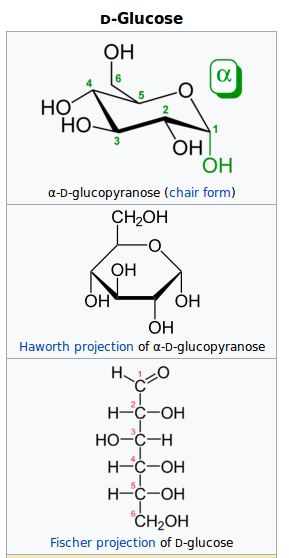
\includegraphics[scale=0.5]{Image/Glucose.png}
& 
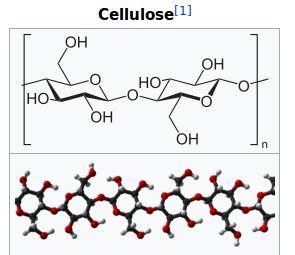
\includegraphics[scale=0.5]{Image/Cellulose.png}
&
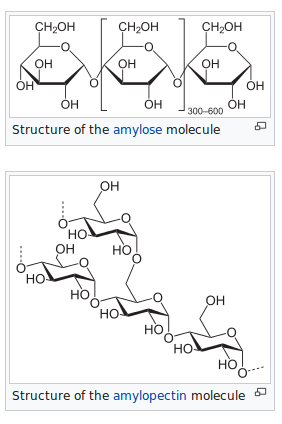
\includegraphics[scale=0.5]{Image/Starch.png} \\  
\end{tabular} 


\paragraph{Polycondensation} \ch{n C6H12O6 -> (C6H10O5)_n + n H2O)} with $n>1000$

There are 2 ways for the liaison. On the top or on the bottom. On the top you get either \begin{itemize}
\item Cellulose : This you can find in straw (paille), gras, wood. We can not eat it since our enzymes can not decompose the bonds, it will not give you energy.
\item Starch (amidon) : This is all we need for "food". Potatoas, wheat, corn.
\end{itemize}
Note that the formula is the same !

Remark that the cellulose can be converted in glucose but it is more complicated than starch. The problem with working with starch is that you compeet with the food market. It does not seem fear to steal the food of someone to create energy to someone else.

The characteristic "biomass" is \ch{CH_{1.6}O_{0.8}} (glucose : \ch{CH2O})
\begin{table}[h!]
\centering
\begin{tabular}{c|c|c}
 & Animal & Plant \\ \hline
Skeleton & bones (\ch{C2CO3}) & lignin \\ 
Body & flesh = proteins  & cellulose \\  
Storage & fat & glucose (also for transportation) \\ 
&& starch (long time)\\ 
&& fat/oils (certain plants)\\
\end{tabular} 
\end{table}



Look at the plant column. We see that glucose, starch and oils, we (human) can eat it. However, cellulose and lignin is not food so we can use it. Nevertheless, it is quiet difficult to do it with lignin.

Characteristic "oil" is \ch{CH_{0.8}O_{0,1}}

The lignin is what is left over if we wait 1000 years, the oil.

The difference between fat and oil is simply that the fat is solid at ambiant temperature and oil is liquid.

\paragraph{Lignocellulose}refers to plant dry matter (\textbf{biomass}), so called lignocellulosic biomass. It is composed of carbohydrate polymers(\emph{cellulose}, \emph{hemicellulose}) and an aromatic polymer (\emph{lignin}).

\paragraph{Comparison with other solid fuels} we start from up right with the glucose a hundred of millions of year ago and now we are with Coal. Note that all fuel on this planet will be on the hachurée area.

\paragraph{Composition and specification of biomass} note that TM is (in german) Dry Matter. This number is really important when you compare biomass with other fuel or even with biomass. You don't need to consider water when comparing. By drinking water, the tree can get some elements. However, only the water evaporates, therefore the other substances (Zn, Mn, Fe, Cu, Cl, and so on) \emph{stay} in the tree. For instance, if we want to use catalyst we will have problem with suffer (\ch{S}) and \ch{Cl} because suffer is a poison for most catalyst. We need to look at the composition of the biomass. This composition depends on \begin{itemize}
\item The type of biomass.
\item The enviromnent of the specific biomass. If the ground is contamined with heavy metal then your biomass will be polluted by heavy metal.
\end{itemize}

%\section{Types and structure of biomass}

\paragraph{Calculation of HHV (Higher Heating Value) /LHV (Lower Heating Value)}
\begin{itemize}
\item example : \ch{CH4} methane = "natural gas" = not biomass
\end{itemize}

We have the following thermodynamics data :
\begin{table}[h!]
\begin{tabular}{c|cccccc}
 & \ch{CH4} & \ch{O2} & \ch{N2} & \ch{CO2} & \ch{H2O} & \ch{N_2} \\  \hline
 $\Delta_f H$ & $\SI{-74.8}{\kilo\joule\per\mol}$ & 0 & 0 & $\SI{-393.5}{\kilo\joule\per\mol}$ & $2 \cdot \SI{-285.8}{\kilo\joule\per\mol}$ & 0
\end{tabular} 
\end{table}

\paragraph{HHV :}\ch{CH4 + 2 O2 + 8 N2 -> CO2 + 2 H2O_{(l)} + 8 N2}
 $$ \Delta H_R = \sum \left ( \Delta_f H_{Produc} - \Delta_f H_{Educ}   \right )  = -\SI{890.3}{\kilo\joule\per\mol}  = HHV$$





\paragraph{LHV :}\ch{CH4 + 2 O2 + 8 N2 -> CO2 + 2 H2O_{(g)} + 8 N2}
\newline
\par
Now we have $\Delta_f H_{\ch{H2O_{(g)}}} = (-\SI{241.8}{\kilo\joule\per\mol})$ due to the following relation

\begin{align*}
 \Delta_f H_{\ch{H2O_{(l)}}} &= \Delta_f H_{\ch{H2O_{(g)}}} - \Delta_{vap} H_{\ch{H2O}} \\
 \Delta_{vap} H_{\ch{H2O}} &= \SI{44}{\kilo\joule\per\mol}
 \end{align*}

Finally we obtain $$LHV =  -\SI{802,3}{\kilo\joule\per\mol}  $$

\paragraph{Remark :}Here we consider that the air is composed of Oxygen (20\%) and Nitrogen (80\%). This explains the stoechiometric coefficients in front of \ch{O2} and \ch{N2}. 

\section{Types and Structure of Biomass}

\begin{itemize}
\item Miscanthus is a typical sort of grass that grows very well.
\item S-Triticale is used to do bread. It is a hybrid of wheat (\textbf{Triti}cum - blé) and rye (Se\textbf{cale} - Seigle).
\end{itemize}

Remind that $ 1 ha = 100 \si{\meter} \times 100 \si{\meter} = \SI{10000}{\square\meter} $

Assume we have global radiation $r \approx 1000 \si{\kilo\watt\per\meter\squared\per\year}$ and the following data

\begin{tabular}{|c|c|c|}
\hline 
S-Triticale & Prod =\SI{9}{\tonne\per\year} & $H_i = \SI{4}{\kilo\watt\hour\per\kilo\gram}$ \\ 
\hline 
Miscanthus & Prod = \SI{10}{\tonne\per\year}  & $H_i = \SI{4.5}{\kilo\watt\hour\per\kilo\gram}$ \\ 
\hline 
\end{tabular} 

Using the fact that $\eta = \frac{(\text{Prod} \times H_i)}{r} $ i.e. the ratio between the energy of we get from the biomass w.r.t. the energy of the sun.

\begin{tabular}{c|c}
S-Triticale & $\eta_T = \frac{ 9000 \times 4}{ 1000 \times 100^2} = 0.36 \%$\\ 
Miscanthus & $\eta_M = \frac{ 10000 \times 4.5}{ 1000 \times 100^2} = 0.45 \%$\\ 
\end{tabular} 

\paragraph{Efficiency} the efficiency is a lot less than photovoltaic but biomass is free, you don't have to buy/construct expensive panel. 

\paragraph{Volume and mass per unit energy of different fuels} the straw can be compressed therefore you gain some volume however you do \emph{not} increase the energy by kilogramm. A kilogramm is a kilogramm, not matter the space it takes. Therefore to go to left in this graph we need chemical process.

Question : why the vegetable oil is not the best biomass ? Looking at the graph it looks like very good. Because it is used for food ! It is attractive to feed our body, to feed the poor people in the world. Besides, taking rapeseed oil (huile de colza) for example, it is a very demanding plant and it needs a rich earth and therefore the capacity is limited.

It is better to use straw because it is a residue from food industry and you can not eat it !

\paragraph{Comparison between energy density per volume between straw and oil}

Taking the data from table~\ref{energy_data} it is difficult to understand since the unit are not the same. We can go further, taking $\SI{2.3}{\tonne}$ of straw we have $\SI{39100}{\mega\joule} $ with a volume of $V = 4.8 \times 2.4 \times 2.25 \approx \SI{26}{\cubic \meter}$ therefore $$ LHV_{straw}= \frac{17\times 2300}{26} = 1500 \si{\mega\joule\per\cubic\meter}  $$

\begin{table}[h]
\centering
\begin{tabular}{|c|c|c|}
\hline 
 & Straw & Diesel \\ 
\hline 
LHV & $\SI{17}{\mega\joule\per\kilo\gram}$ & $\SI{36000}{\mega\joule\per\cubic \meter}$ \\ 
\hline 
\end{tabular}
\label{energy_data} 
\caption{Energy data}
\end{table}



It follows that $$ \SI{1}{\cubic\meter} \text{Diesel}= \SI{24}{\cubic\meter} \text{straw}$$ 


\paragraph{Remark}that you need to check that your truck does not consume more energy that it is carrying ! Therefore you need to take shorter distance or process your straw !
This is for volume, for masse we have a factor of 2 and not 24.


\section{Fuels from oil seeds}
\paragraph{Comparison of liquid (bio) fuels}
You can find on FNR.de This is a comparison of how much km I can do with 1 ha of farmland. Don't need to know the number of course.
\paragraph{Remark}that even if Rapeseed oil has a more energy density, it is less efficient as straw. Therefore BtL is more efficient as Rapeseed ! The reason come from the fact that to get the oil, you just need the seeds. However for BtL you eat the seeds and can use all the rest to produce bio diesel.

\paragraph{Remark}that on average a german travel about \SI{20000}{\kilo\meter} a year. 

\paragraph{Palm oil}is very efficient however this does not make sense to cut the rain forest to grow palm oil when the aim is to reduce the carbon impact of energy. Notice that it is caused by bio diesel but also for food !

\paragraph{Structure of oils and fats}which are triglyceride (triester of glycerin=glycerol) of fatty acids (carboxylic acids).


\paragraph{\color{red}{tri}\color{violet}{glyceri}\color{green}{de} \color{black}{of} \color{blue}{fatty acids}} 


\begin{itemize}
\item[\textbf{\color{violet}{Glycerine}}]is an alcohol of 3 \ch{OH} groups. Below you find the lewis structure (left) and the same structure without the carbone atoms (right).

\begin{tabular}{cc}
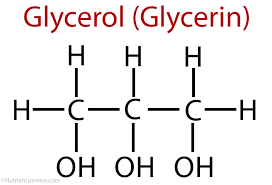
\includegraphics[width=0.5\textwidth]{Image/glycerine1.png} & 
\includegraphics[width=0.5\textwidth]{Image/glycerine2.png}
\end{tabular}

\item[\textbf{\color{blue}{Fatty acids}}] are \textbf{carboxylic acids} with a long \textbf{aliphatic} chain, in natural form they have an \textbf{even} number of \ch{C}-atoms from \textbf{4 to 28}.

\paragraph{Carboxylic acids}is an organing compound that contains a \textbf{carboxylic group} \ch{COOH}. The general formula is $$ \ch{C_n H_{(2n+1)}COOH} $$. The first ones can be seen on Table~\ref{carboxylicacid}. 

\paragraph{Aliphatic compound}any chemical compound belonging to the organic class in which the atoms are not linked together to form a ring.

\paragraph{Saturated fatty acids}are the so called carboxylic acids containing \ch{C=C} double bond.

\begin{figure}[h!]
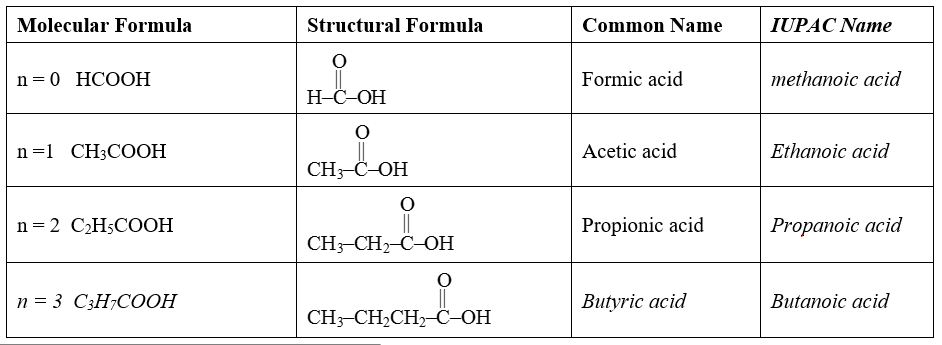
\includegraphics[width=\textwidth]{Image/carboxylic-acid-formula.png}
\caption{First carboxylic acids.}
\label{carboxylicacid}
\end{figure}

The fatty acids have always an \textbf{even} number of C-atoms . If you spill this acid in the nature, the ground, the tree are going to eat it. You can also drink it. However, if you spill acid with \textbf{uneven} number of C-atoms, the nature will not consume it. This is the reason why you can not spill fossile fuel : it has uneven C-atoms. 

\item[\textbf{\color{green}{Ester}}] = Alcohol - carboxylic acid (Alcohol bounded with fatty acid)

The simplest ester is the simplest alcohol with the simplest carboxylic acid \[ \ch{CH3OH + HCOOH -> HCOOCH3 + H2O} \]

i.e. Methanol with formic acid gives Methyl formate and water.
\begin{table}
\begin{tabular}{cc}

\includegraphics[width=0.3\textwidth]{Image/mthanol.png} & 
\includegraphics[width=0.5\textwidth]{Image/methyl_formate.png}
\end{tabular}
\caption{Left methanol and right Methyl formate}
\end{table}

\end{itemize}

Finally we can create our triglyceride (triester of glycerol) of fatty acids. We take an alcohol (glycerine) and {\color{red}\textbf{three}} fatty acids and we get our product

\begin{figure}[h!]

\includegraphics[scale=1]{Image/oilandfats.png}
\caption{Here $R^{'}$,$R^{''}$ and $R^{'''}$ have 13 to 21 $\ch{C}$ such that the whole fatty acid is $\ch{C_{14-22}}$. Notice that 3 \ch{H2O} are created in this process. Indeed, the 3 \ch{OH} groups of the glycerol merge with the 3 \ch{H} of the carboxylic group \ch{COOH}.}
\end{figure}



\paragraph{Remark}for our calculation (and for the exam) only double bonds, not \ch{OH} groups or EP.

\subsection{Fuels from oil seeds}

\paragraph{Problem with Rapeseed} We want our \emph{biodiesel} to be \emph{compatible} with the actual engine. Otherwise nobody is going to buy our fuel. We therefore need to fulfill all the criteria of \emph{diesel}.

\begin{itemize}
\item \textbf{Viscosity} of Rapseed oil is to high, it should be less than \SI{10}{\square\milli\meter\per\second}. 

\item \textbf{Cetane} number has to be at least 50. Cetane number, Cetane rating or CN is an indicator of the combustion speed of diesel fuel and compression needed for ignition. 

\item \textbf{Flammability} point is too high.

\end{itemize}

The last point to take into account is the fuel equivalent. You consume 4\% more with Rapsöl (i.e. Rapeseed, i.e. colza) than with diesel. This is a \emph{financial} problem.

Therefore we need to convert our oil in something else : the \textbf{Biodiesel}.

\subsection{What is bio diesel ?}
If you start form Rape (also known as Rapeseed and in French \textbf{colza}) you get \textbf{RME}, if you start from any kind of oil you have \textbf{FAME}.

\paragraph{FAME Process}involves the cutting of the molecule in 4 smaller molecules : therefore the viscosity drops and the flammability goes down.

\begin{figure}
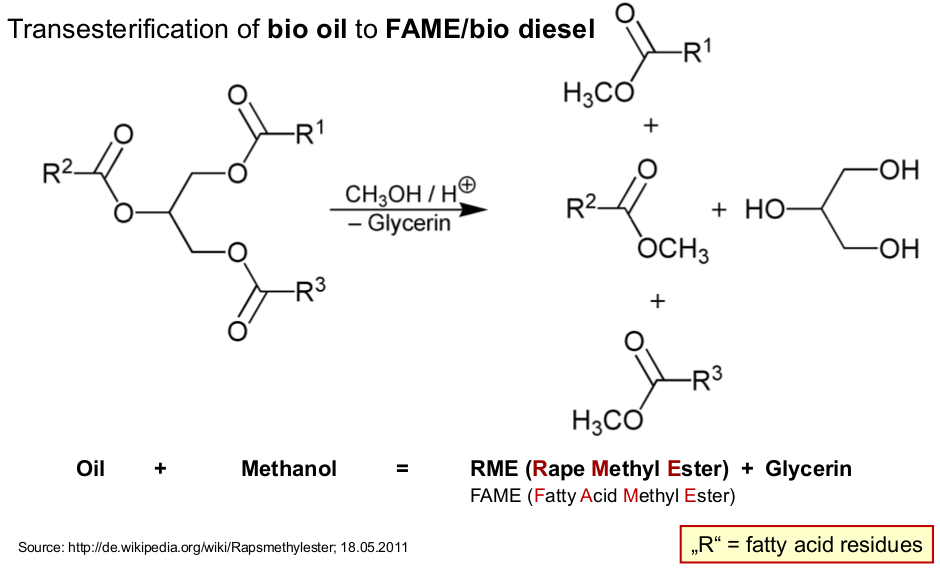
\includegraphics[scale=0.5]{Image/FAME.png}
\end{figure}

\paragraph{Problem}Usually in your car, you have plastic in the fuel system (e.g. the tank, the pipes), and the poor bio diesel destroys the plastic. Thus you need to change the tank, the piping etc. Otherwise, you can mix the biodiesel with fossil diesel and then you do not dammage your plastic. This is done in germany about 10\%.

However you need to take into account the fact that to grows your plant you need fertiliser, fuel to harvest etc. At the end of the day, for 10\% mix of bio diesel, it reduces the fossil fuel from 4 to 5\%. This is not enough.

\paragraph{HVO (=alternative to FAME)}(\textbf{H}ydrogenated \textbf{V}egetable \textbf{O}il) Let us first totally hydrate or triglyceride of fatty acids.


\begin{tabularx}{\textwidth}{  X  r  X }
  \noindent\parbox[c]{\hsize}{\chemfig{C(-[:0]{\color{violet}{\color{violet}O}}(-[:0]C(=[:90]\color{violet}{O})(-[:0]R_1)))(-[:90])(-[:180])(-[:270]C(-[:0]{\color{violet}O}(-[:0]C(-[:0]R_2)(=[:45]\color{violet}{O})))(-[:180])(-[:-90]C(-[:180])(-[:-90])(-[:0]{\color{violet}O}(-[:0]C(=[:-90]\color{violet}{O})(-[:0]R_3)))))} } & $+ \ch{12 {\color{orange}H2}} \ch{->} \ch{6 {\color{orange}H2}{\color{violet}O}} + \sum_{i=1}^3$ \chemfig{C(-[:0]R_i)(-[:90]\color{orange}{H})(-[:180]\color{orange}{H})(-[:-90]\color{orange}{H})} $+$& \noindent\parbox[c]{\hsize}{\chemfig{C(-[:0]\color{orange}{H})(-[:90])(-[:180])(-[:270]C(-[:0]\color{orange}{H})(-[:180])(-[:-90]C(-[:180])(-[:-90])((-[:0]\color{orange}{H}))))}}  \\
\end{tabularx}

\begin{itemize}
\item[Advantage] : can be directly substituted as diesel. Does not contain any aromatic component and sulfur. Yield more then 85\% of ma.-\% (mass fraction).
\item[Disadvantage] : it needs a lot of dihydrogen (12 mole for one mole of fat oil) and this dihydrogen is expensive and comes up to now from fossile oil. Moreover, this big molecule becomes solid when the temperature goes down. This is very nasty for plane. For plane you cut the big ones (you cut the \ch{C_{14} - C_{22}}. It also has a poor stabililty under low temperature. 
\end{itemize}

\paragraph{Remark} CoMo or NiMo are catalytic. There is 2 ways of doing it, Hydrogenation or Blending.

\begin{itemize}
\item[Hydrogenation]
\item[Blending]
\end{itemize}
\paragraph{\color{red}{Exam Question}}Compute how much dihydrogen you need to completely hydrate a molecule similar to the oil

\paragraph{Biodiesel}can be for example B7 (7\% of biodiesel) or B100 (100\% of biodiesel).

\paragraph{Byproducts}produced by \textbf{HVO} process are \ch{H2O , C3H8 , H2S , NH3}

\section{Fermentation to Ethanol}
The \emph{ethanol} is a substitute to \emph{gasoline} - while \emph{biodiesel} is a substitute to \textit{diesel}. 
\subparagraph{Sugar} Two suitable (sugar) plants for ethanol production.
\begin{itemize}
\item \textbf{Sugar beet}
\item \textbf{Sorghum}
\end{itemize}
\subparagraph{Starch} the suitable (starch) plants for ethanol production.
\begin{itemize}
\item \textbf{Potato}
\item \textbf{Topinambur}
\item \textbf{Grain}
\item \textbf{Corn}
\end{itemize}
\paragraph{Drawback of bioethanol}there is a limitation. You can used only plant with \emph{sugar} or \emph{starch}. Thus you compete with the food industry.

\paragraph{Formation}can be shown in the following equation. Notice we take a macro point of view and consider glucose.

\begin{tabular}{cccc}
\ch{C6H12O6_{(aq)} &->[yeast] & 2 CH3CH2OH(l) + & 2 CO2(g)} \\
starch & & EtOh - Ethanol & Gaz
\end{tabular}

\begin{itemize}
\item[Problem I :] The maximum of Ethanol concentration that you can have is $x_{EtOH} \approx 10 Vol.\%$ this is due to the fact that the ethanol kills the yeast (levure). This is the reason why a typical wine bottle is 10\%. However the aim for fuel is $x_{EtOH}>99 Vol.\%$. We therefore need distillation/rectification.
\item[Problem II :] Tank or table ? Is it really good to use sugar which could feed people ?
\item[Problem III :] Tank or table (bis) ? Is it really good to use starch which could feed people ?


\begin{table}[h!]
\centering
\begin{tabular}{ccc}
\ch{ (C6H10O5)_n + & n H2O &->[cheap\,enzyms] n C6H12O6} \quad \text{with} $n > 1000$ \\
starch & &
\end{tabular}
\end{table}

\item[Problem III :]The cost of Ethanol is at now higher than gasoline and it is a less efficient fuel, you can drive less with than with gasoline. Thus you need either to put it at lower price (via state incentive) or penalize people buying gasoline.

\item[Advantage I :]The octane number is greather than 100 which is quiet nice !
\end{itemize}

\paragraph{It would be nice} if the ethanol was formed from grass and trees but at now it is the case only in laboratory.

\paragraph{Use of i-Butylene}This by product of refinery can be used. This is a byproduct in the cracking of crude oil product.

\begin{figure}[h!]
\centering	
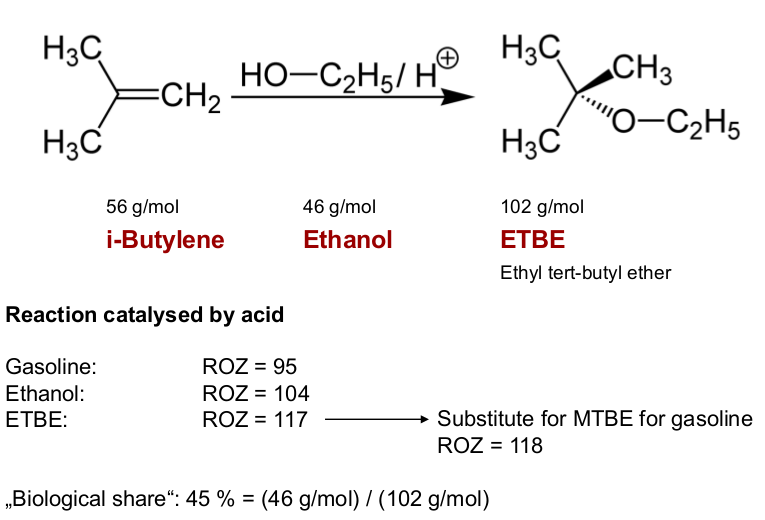
\includegraphics[scale=0.5]{Image/iButylene.png}
\caption{Note that ROZ is the octan number.}
\end{figure}

\paragraph{Ether} is a molecule with a \ch{O} as link.

\paragraph{ETBE} is a high value product (high ROZ = High octane number). So the refinery was doing it \emph{before} the urge to make more green product.

\paragraph{Biological share}Let's take the ETBE. It comes from ethanol (biomass) and i-butylene (fossil fuel) and can not be considered as 100\% from biomass. The biological share is in that case $\frac{46}{46+56} \approx 45 \%$

\paragraph{Improved process}At now the plant as an efficiency of about 30\%. Indeed, it needs a lot of energy for the destillation process and also for the drying to create \textbf{DDGS}. However one can reach an efficiency of 50\% by also creating biogaz as byproduct.

\subsection{Fuel application of EtOH}

\begin{itemize}
\item Direct mixture with gasoline
\item Conversion to ETBE and mixture with gasoline.
\item (use of pure EtOH). This need a change in all the pipe and tank of your car.
\end{itemize}

\paragraph{Competitivity} the ethanol is at now twice the price as gasoline but the government skips the taxe for fuel and therefore it can be competitive. 

 \paragraph{Gasoline vs. Bioethanol} looking at table "properties of selected bio fuels", wee that everything is ok except the energy equivalence, you need nearly twice as much as bioethanol than gasoline e.i. bioethanol will propably be more expensive.
 



\section{Biofuels}
\subsection{Introduction and motivation}
\paragraph{Motivation}
\begin{itemize}
\item It exhibits the highest energy density today
\item It has the potential of greenhouse gas savings
\item Now producing biofuel is more expensive than producing fossil fuel. We need \emph{state incentives}.
\end{itemize}
\subsection{Type of biofuels}
\paragraph{First Generation} \emph{State of the art}
\begin{itemize}
\item Ethanol from sugar/starch
\item Biodiesel from Rape, soy bean, palm oil, Jatropha : HVO and FAME
\item HEFA (Hydro-processed esters and Fatty Acids)
\end{itemize}

Remark the advantage of Jatropha is that it can grows on low quality land however the farmer will try to grows it on rich land and therefore will compeet with the food. Table or tank ?

\paragraph{Second Generation} \emph{Development}
\begin{itemize}
\item Synthetic fuels (BtL)
\item Alcohol from cellulose
\end{itemize}

Here we use residues from agriculture and forestry as well as waste.

\paragraph{Third Generation} \emph{Research}
\begin{itemize}
\item Microbial fuels
\item Micro algae
\end{itemize}

\subsection{Second Generation synthetic biofuels}

Ligno cellulosis biomass \ch{C6H9O4} this molecule will be synthetised in \ch{H2 + CO}.

\paragraph{Fischer Tropsch Synthesis} here syngas is transformed in hydrocarbures. Remark you get all these product at the same time :\begin{itemize}
\item Gases : Ethylene,...
\item LPG : Liquid Propalined Gaz : ex for camping
\item Naphta
\item Cerosene : Jet Fuel
\item Diesel 
\end{itemize}
However the lubes and waxes are not really interesting byproducts. One can increase its  interesting products (LPG, naphta, Diesel) with \textbf{hydrocracking}. However it needs a higher effort in downstream processing.
\paragraph{\ch{H2 + CO}} We can create methane with the following reaction

\ch{CO + 3 H2 ->[cat.]  CH4 + H2O}

Remark that this is the future, when we won't have anymore natural gazes. This is called SNG (Substituted Natural Gaz)


The advantage of this equation is that in Europa we have a very nice pipeline system. Therefore you can easily travel it from Netherland to spain etc. This is not the case in the east (ex. Russia ?).

The drawback is that you transfer some of your valuable hydrogren into water...

\paragraph{Hydrogen as the future} \ch{CO + H2O ->[cat.] H2 + CO2}

You can get rid of the \ch{CO2} using CCS (Carbon dioxyde Capture and Storage). The idea is to store it underground.

\paragraph{Going to Methanol} this is according to the KIT very promising.

Methanol itself is a very useful product. For example you need it to create biofuel (biofuel is 90\% of (?) and 10\% of methanol). In Germany you can not put more than 10\% of methanol, it is prohibited because it becomes a poison (?)

\subparagraph{Dimethylether DME} is a process to transform methanol into fuel that you can use.

\ch{2 CH3OH -> CH3OCH3 + H2O}

From this molecule you can form PE (polyethylene) and PP (PolyPropylene) which create a lot of the plastic today.

$$ PE = \ch{C = C} $$
$$ PP = \ch{C-C} $$

\paragraph{SUIT} the suit is a molecule of C :

\ch{C-C-C-C-C-C-C}

this is the reason why the oxygenated fuel like Methane, Methanol form not so much of suits. 

\paragraph{FischerTropsch synthesis} was very used in south africa the reason is that because of the embargo, they were not allowed to import crude oil. Thus they used that process to produce crude oil.

Without Hydrocracking you have a lot of heavy hydrocarbure like Lubes and Waxes. The hydrocracking breaks theses molecules.

\subparagraph{Economics} a barrel is $\approx$ 160 liters, bbl/d is barrel per day. On the slide you see that the investment price per barrel changes a lot ! A factor if 6 for the last 2. It shows that it is very difficule.

\paragraph{Characteristics of synthetics Xtl-fuels}
This synthetic (liquid) fuels are more cleaner (form less fuels, you can find it on the picture, the more it glows, the more it forms suits).

Remark, fuel that are directly fully compatible to existing conventional fuels are called "Drop-in fuels".

\paragraph{Potential feedstocks} this methods avoid competition with agriculture.

\begin{itemize}
\item Residue, etc straw
\item Energy crops (example China grass, it is kinda big (4m) you cut the half and let the rest grows)
\item Stumps and tops (residues from forest)
\end{itemize}

\paragraph{Large scale use of lignocellulosic biomass}

\subparagraph{Economics reminder} suppose that you have 2 plants, one is twice bigger.

\[ C_2 = C_1 \left(\frac{S_2}{S_1} \right)^n \quad n < 1 \]
$n$ is the disgression parameter. The more you produce, the easier you produce.

However, you need to take into account the transporation because the bigger is your plant, the further your plant needs to be.

 Therefore there is an optimum. This is the reason why most of these 2sd generation plant are $\approx$ \SI{200000}{\tonne \per \year} $\approx$ 30-50 \si{\kilo \meter}. This number needs to be taken into account with the traditional plant (not from biomass) $\approx  $  \SI{15}{\mega\tonne \per \year}, this is the reason why from economy scale reason, biomass is more costy. A solution may be to increase the energy density of your fuel. With that you can reach \SI{1,5}{\mega\tonne \per \year} however you still have an increase of costs from the increasing of energy density.
 
 
 \paragraph{Straw in Europa}
 \begin{itemize}
 \item You see that there are area with a lot of straw mainly in France. We also see that even if there are 150 M tonne per year, we could probably used a third of it to produce biofuel.
 \item There is no global market for straw, even no continental market, only national market. However, if we use straw to produce energy, the price will probably harmonize to the price of the energy it contains. (This phenomenon can be seen in Germany with Food pallet used to heat).
 \item An other issue is the fact that the harvest depends on the year. Even if it globally increases through the year, you can have a bad year, ce qui est chiant pour le feed stock planning.
 \end{itemize}
 
 \subsection{Third Generation: Algae for fuel production} the idea ist to use algae to synthetised our fuel, we have the following production system
 \paragraph{Open ponds}is a large circular pool
 \paragraph{Raceway ponds}is divided into rectangular grid
 \paragraph{PBR}Photo BioReactors gives a better energy yields by illuminating the algae and circulating it. Indeed, too much light kills the algae and too many also lead to the death of the algae.
 
 \paragraph{Open bonds vs. PBRs} Let us compare both
 \begin{table}[h!]
 \centering
 \begin{tabular}{c|c}
 \textbf{Open ponds} & \textbf{PBR} \\ \hline
 {\color{green}Low} construction costs & {\color{red}High} construction costs \\
 {\color{red}Low} cell concentration & {\color{green}High} cell concentration \\
  {\color{red}High} risk of biological contamination from environment & {\color{green}Low} risk of contamination\\
   {\color{red}High} water consumption (evaporation) & {\color{green}Good} process control \\
  {\color{green}Easy} scale-up & \\
 \end{tabular}
 \end{table}

This process is still using a lot of energy and has an \textbf{EROI} (Energy return of invest) of $\approx 1$.

\paragraph{In the future}one can genetically modify the algaes such that it produces from \ch{CO2} some fuels. We can already produce ethanol by photosynthesis. 
 
\section{Fermentation and upgrading to biogas}
 \subsection{Fermentation to Biogas}
 \paragraph{Material needed}in order to form biogas, you can use any energy crops, organic waste or manure. Note that one could also use wood or straw but then the process is \emph{not} very efficient/interessant.
 
 \paragraph{Bio SNG}Bio substituted/synthetic natural gases. 
 
 \paragraph{Bio mass: Introduction and statistics}you can see that now (2013), biomass has a quiet large share of the \textbf{Power} sector (27.2 on 150.9 \si{\tera\watt\hour}, a not so bad in the \textbf{Heat} Sector (11.5 on $\approx 130$ \si{\tera\watt\hour})
 
 \paragraph{Biogas - the way of the nature}the \textit{cow machine}. Some people say that the cows have the same impact on the climate that the world traffic.
 
 \paragraph{Chemistry point of view}\ch{C6H12O6 ->[Archea, H2O] 3 CH4 + 3 CO2} useful for us is only the mycene.
 
 The Archea are converting our glucose to biogas. Why are they doing it ? Because they get energy from this reaction. The reaction balance can be understand using the intermediate steps.
 
 \begin{itemize}
 \item \textbf{Fermentation to acetate} \ch{C6H12O6 + 2 H2O ->[\SI{-216}{\kilo\joule\per\mole}] 2 CH3COOH + 2 CO2 + 4 H2} \\
 We produce acetic acid.
 \item \textbf{Methanogenesis} (by archea) \ch{2 CH3COOH + 2 CO2 + 4 H2 ->[\SI{-202}{\kilo\joule\per\mole}] 3 CH4 + 3 CO2 + 2 H2O}
 \end{itemize}
 
 Summing up we obtain \ch{C6H12O6 ->[\SI{-418}{\kilo\joule\per\mole}] 3 CH4 + 3 CO2} the energy of \ch{CO2} is zero and when you look at your balance of energy, you see that 15\% of the energy is lost in the process and therefore 85\% is in the \ch{CH4}. This is a \emph{huge} efficiency process. 
 
 \begin{equation}
 \label{Rendement}
  \eta = 1- \frac{\text{Lost energy}}{\text{Total energy}} = 1 - \frac{418}{3 \times LHV + 418}= 14.8 \% 
 \end{equation} 
with $LHV = \SI{800.9}{\kilo\joule\per\mole}$.
\paragraph{Remark}everything from biomass can be fermented except the lignin. The reason we do not use wood and straw is because it has a lot of lignin.

\paragraph{Biogas yields} you should know that out of 1 tonne of Maissilage, you get \SI{200}{\meter\cubed} biogas $\approx$ \SI{100}{\meter\cubed} \ch{CH4}.

\paragraph{Number of plants}Germany is the country which has the most biogas plant, up to 9000. However, on the 9000, more or less 8000 are just small plant using the material on the right of the slide Biogas yields. In fact, one needs to get rid of the poop of the cows, however one can still extract a little bit of energy by forming biogas. Note that it is ok because cows are in stable (étable).

\paragraph{Remark on the smell} Normally in the product your reactifs also have protein that contains for instance \ch{S}. Therefore at the equation reads 
$$\ch{\text{Protein} + C6H12O6 ->[Archaea, H2O] 3 CH4 + 3 CO2 + H2S + NH3}$$

The problem with \ch{H2S} is that if you burn it you get :
$$\ch{H2S -> SO2 + H2O}$$

\paragraph{Potential and limits} 1 hA of biogas is enough to satisfy the eletricity demand of 5 german households during a year.

\paragraph{Mycene vs Carbone dioxed} the mycene is 20 times higher as Carbon dioxed for the climate.

\paragraph{Process Conditions} do not learn all the number by heart. Just to know that best temperature is \SI{40}{\degree}
\paragraph{Material to create biogas}
\begin{itemize}
\item Glucose : Food {\color{red}ko}
\item Starch : Food {\color{red}ko}
\item Cellulose {\color{green}ok}
\item oil/fat : Higher value than biogas {\color{red}ko}
\item Lignin : Not working {\color{red}ko}
\end{itemize}

\paragraph{Cellulose fermentation to Biogas}\ch{(C6H12O5)_n + n H2O -> n C6H12O6 ->[\text{Archaea}] 3 CH4 + 3 CO2 (+ H2S + NH3)}

with the following parameter :

\begin{itemize}
\item Temperature. $T$ is in the range 20 to 50 degree. Thus in average 40\si{degree}C.
\item Time. $\tau$ is more or less 30 days, therefore the volume of the reactor should be able to carry 30 days of production.
\item $x_{\text{solid}} < 15 \% \Rightarrow x_{\ch{H2O}}> 85 \%$
\item 1t of fresh material (corn silage) gives 200$m^3$ Biogas gives 100 si$m^3$ of \ch{CH4}
\end{itemize}

\paragraph{Problem with \ch{H2S} and \ch{NH3}} with oxygen this gives

\begin{align*}
\ch{H2S + 1.5 O2 &-> SO2 + H2O} \\
\ch{2 NH3 + 2.5 O2 &-> 2 NOx + 3 H2O}
\end{align*}

\paragraph{Problem with CHP}the efficiency is too low because you have an efficiency of 25 to 45 \% to electricity. It rests thus 55 to 75 \% of heat. However, what do you do of the heat in summer ? And most of the time these plants are in the middle of nowhere. Therefore you lose more than the half of the energy. Also, you need to be connected to the power grid.

\subsection{Upgrading of biogas to substitute natural gas (SNG)}

\begin{tabular}{|c|c|}
\hline 
bio SNG & bio Synthetic Natural Gas \\ 
\hline 
• & bio Substitute Natural Gas \\ 
\hline 
• & bio Methane, green Methane \\ 
\hline 
\end{tabular} 


\paragraph{Technical System (slide)}If we can not use the waste heat of the CHP we get an efficiency of 35\%. On the other hand, if you have the possibility to use all the heat, you reach 76 \%. In Germany 8800 plants do that.

However, if you use upgrading, then the efficiency is $\approx 65 \%$. More or less 200 plants in germany do that.

To summarize, if you can use all the heat, you should do the CHP; if you can not use the heat but you can connect to the gas grid then you should do upgrading. Finally, if you can not connect to the gas grid but you can connect to the electrical grid, you should do the CHP.

\paragraph{Upgrading of Biogas}this process is very sensitive. This is a living system, a living reactor. It reacts differently during day and night or if it rains or not.

\paragraph{Parameter}

\begin{itemize}
\item $H_s$, heating value; energy content of the gas. You see that you are between 5 and 7.7 however the germany standard is 8,4. Even the best plant does not reach this standard.
\item \ch{CO2} (dry) : it also does not reach the standard in Germany.   
\item Same for \ch{H2S} (dry) and \ch{H2O}
\end{itemize}
You therefore need to do a lot of transformation to reach the standard.

\paragraph{Primary desulfurization} \ch{FeCL2 + H2S -> FeS + 2 HCl} The \ch{HCl} stays in the water increasing the pH but it is not a problem since we are talking about a few ppm. Doing this you can remove a big amount of the sulfure but not totally, and it is still too high so you need other way.
\paragraph{WTF} we have an efficiency of 85 \% of \ch{CH4} and after upgrading we get 65 \% (due to the fact that the upgrading consumes energy).

\paragraph{Upgrading by physical scrubbing} First you compress then you remove water. Then it goes to a scrubber. You put pressurized water (8 bar) at the top and the water goes out at the bottom as sparkling water. (Do not care about the flash). Remark the lean gas is mainly \ch{CO2}. This is a continuous process.

You can do it with Water or with genosorb (better but more expensive). You can see it in Henry's law.

This process works because \ch{CO2} and \ch{H2S} are more soluble in water than methane. Therefore the methane is in gas phase while the latters are on liquid phase.

\begin{itemize}

\item High pressure and low temperature gives \textbf{absorption} of carbone dioxyde and also other gases if they are still there (ex. \ch{H2S}) but not of \ch{CH4}.
\item Low pressure and high temperature\footnote{remark that most of the people do not rise the temperature since it is expensive and it works enough without.} gives a \textbf{desorption} of \ch{CO2}
\end{itemize}

Here you need to increase the pressure, you need a compressor, you need \textbf{electricity}.

\paragraph{Chemical scrubbing} in this case the pressure is irrelevant. However you do use water, you use complicated and expensive solvant. On the other hand you get a very pure product (99\%)

\begin{itemize}
\item Low temperature means \textbf{absorption} of \ch{CO2}
\item High temperature means \textbf{desorption} of \ch{CO2}
\end{itemize}

Here you need to increase the temperature, you need \textbf{heat}. You can use fuel or waste heat. For instance, you can do a little part of CHP. You sell the electricity and use the heat. This makes sense only in big plant.

\subparagraph{What is the chemical reaction ?} You have a chemical reaction between gas and liquid, for instance one can use Potassium. 
\begin{align*}
\ch{K2CO3(aq) + H2S(g) &->[T \text{low}] KHS(aq) + KHCO3(aq)} \\
\intertext{and the other way}
\ch{K2CO3(aq) + H2S(g) &<-[T \text{high}] KHS(aq) + KHCO3(aq)}
\end{align*}
Notice that the equilibrium constant, and therefore the direction of the reaction (direct or inverse) depends on the thermodynamics.

\paragraph{General remark on scrubing} one needs 2 reactions because we want to reuse our solvent. The first reaction is the separation between methane and the other gases, the other one is the separation of the other gases and the solvent. 
\paragraph{Reminder on \textbf{ad}sortion} En chimie, l’adsorption est un phénomène de surface par lequel des atomes, des ions ou des molécules (adsorbats) se fixent sur une surface solide (adsorbant) depuis une phase gazeuse, liquide ou une solution solide. Dans le cas d'un atome adsorbé, on parle d'adatome. Ce phénomène ne doit pas être confondu avec l'absorption dans lequel un fluide ou le composant d'une solution solide est absorbé dans le volume d'une autre phase liquide ou solide.\cite{wiki_adsortion}
\paragraph{Pressure swing adsortion}
TODO
\paragraph{Upgrading with membrane}some polymere can separated the \ch{CO2} and \ch{CH4}. One needs a step of compression and, of course, this seperation is not perfect. This is the reason why you do more steps. At least 2 steps.

The drawback is that this membrane is intolerrant to S-species (e.g. \ch{H2S}). It is killed by the sulfure, and it is expensive ! Thus you need a desulfurization before.

Up to now there are 4 or 5 plants working with this technology. Again compressor is electricity.

\newpage

\bibliography{mybib}

\bibliographystyle{plain}

\end{document}
